We developed a semi-structured interview protocol to explore how educators
across a variety of tertiary insitutions. In
Section~\ref{subsec:interview-questions}, we describe the interview questions
that we developed and in Subsection~\ref{subsec:interview-probes} we describe
the taxonomy of interview probes we empoloyed to guide consistent follow-up
questions across interviews. Following this, in
Section~\ref{sec:data-collection} we describe our recruitment and data
collection procedures. Finally, in Section~\ref{sec:data-analysis} we describe
our approach to analyzing the data collected through these interviews.

\begin{figure*}[ht]
  \centering
  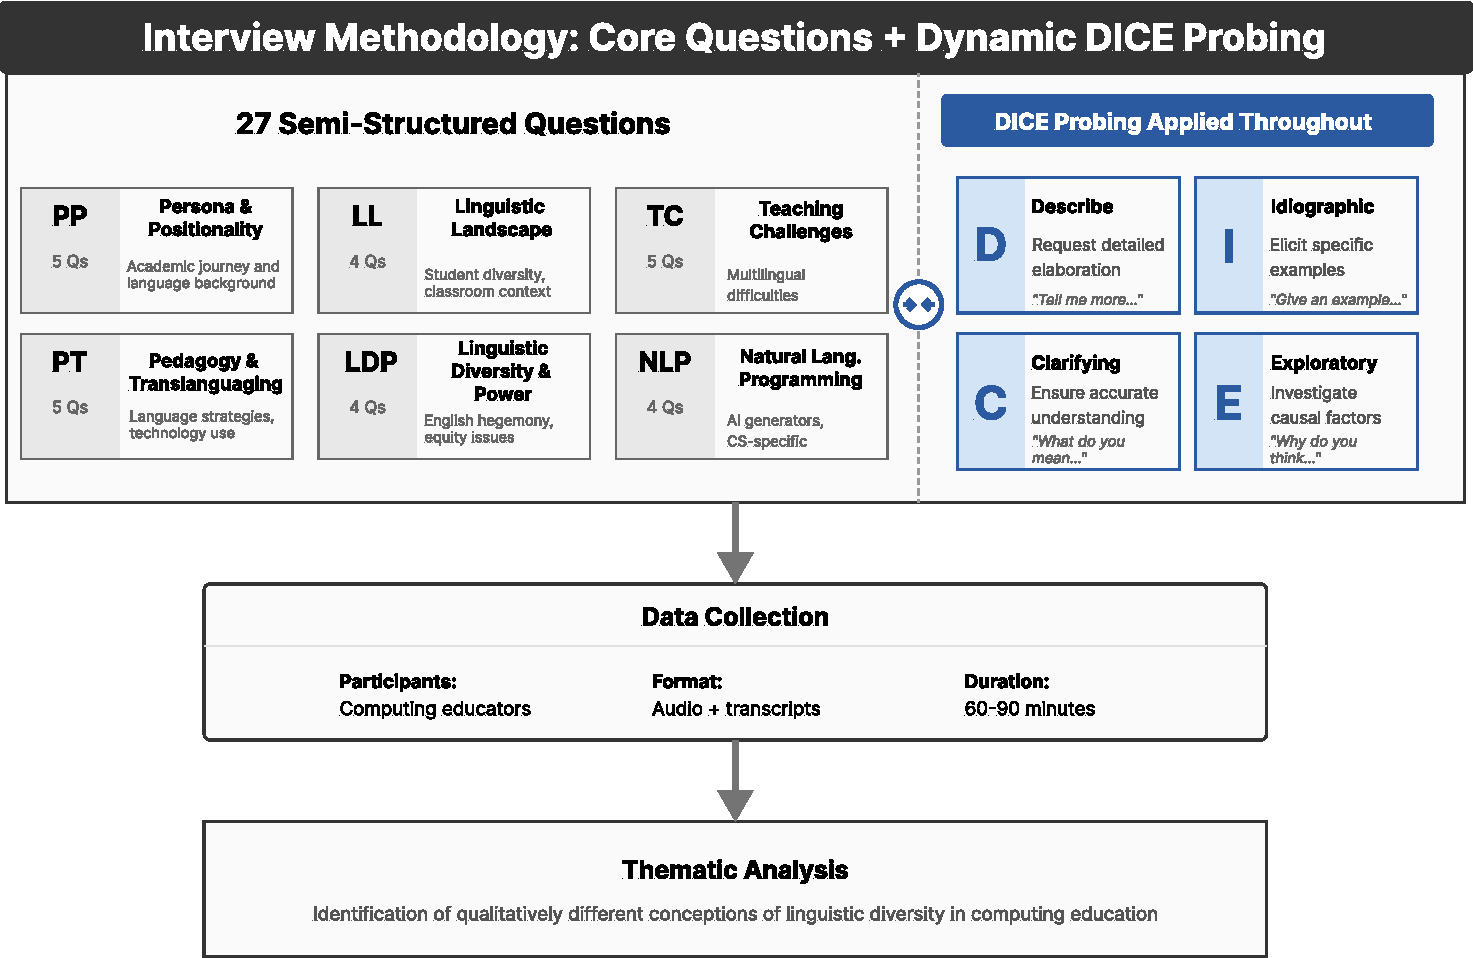
\includegraphics[width=\textwidth]{imgs/methods.pdf}
  \caption{Your caption here.}
  \label{fig:methods}
\end{figure*}


\subsection{Interview Questions}\label{subsec:interview-questionse

\subsubsection{Persona and Positionality}\label{subsubsec:persona-and-positionality}

% Context and grounding
Given the phenomenographic nature of this work, it is important that we
understand the context and positionality of each participant. These questions
are designed to provide this context---with particular focus on the
educational, instructional, and linguistic backgrounds of each participant. 
\begin{enumerate}[label={PP.\arabic*}, align=left, leftmargin=4em]
  \item Could you briefly describe your academic journey and how you came to
    teach in your current position?
  \item What subjects do you currently teach, what levels (e.g., undergraduate,
    graduate) are these courses, and in what contexts (e.g., in-person, online,
    hybrid) are they delivered?
  \item What languages do you speak, and in what contexts do you typically use
    each?
  \item In your own education, what language(s) were used for instruction?
  \item What are your general thoughts and beliefs about the role of language in
    education, particularly in technical fields like computer science?
\end{enumerate}

\subsubsection{Linguistic Landscape}\label{subsubsec:linguistic-landscape}

Informed by the work of \citet{gorter2021linguistic}, we aim to understand the
``linguistic landscape''---which refers to the outward display of languages in
public spaces---of the context in which participants teach and any potential
mismatches between the languages spoken by students and those that are visible
in the learning environment. To this end, we ask the following questions:
\begin{enumerate}[label={LL.\arabic*}, align=left, leftmargin=4em]
  \item How would you describe the linguistic diversity of your current students? 
  \item In your experience, what is the range of proficiency in English---or your primary medium of instruction---among your students? 
  \item How visible are different languages in your in your classroom materials, textbooks, documentation, and physical/digital learning spaces?
\end{enumerate}
Responses to these questions aim not only to understand the participants
linguistic environment but also to contextualize responses to questions in the
following sections. This aims to offer the interviewer a better understanding
of the participants context and enabling them to ask more informed follow-up
questions.


\subsubsection{Teaching Challenges}\label{subsubsec:teaching-challenges}

Empirical work has consistently found that teaching in a multilingual environment
presents unique challenges which are often unaddressed in teacher training and
professional development programs at the K-12 level~\cite{}. Such challenges may
be more pronounced in higher education, where instructors may have even less
explicit training in pedagogy~\cite{}. To understand the emergent challenges we
ask the following questions:
\begin{enumerate}[label={TC.\arabic*}, align=left, leftmargin=4em]
  \item What challenges, if any, do you face teaching topics in computing to
    students who speak a variety of languages?
  \item Can you describe instances where you felt language background created a
    barrier to student learning or engagement in your classes?
  \item When, if at all, have these challenges been addressed in any formal
    training or professional development programs for teaching you've
    participated in?
\end{enumerate}
Responses to these questions aim to uncover not only the challenges that instructors 
face but also provide potential avenues for follow-up questions in the sections
that follow for how instructors navigate these challenges in practice.


\subsubsection{Pedagogy and Linguistic Diversity}\label{subsubsec:pedagogy-and-translanguaging}

In this section, we explore the pedagogical strategies employed by educators 
to navigate linguistic diversity in their classrooms. Drawing on the principles
from translanguaging~\cite{}, code-switching~\cite{}, and critical language awareness~\cite{} we ask the following
questions:
\begin{enumerate}[label={PT.\arabic*}, align=left, leftmargin=4em]
  \item How do you decide when to use a particular language for
    instruction or explanation during your classes and when, if at all, do
    to change languages?
  \item If you've adopted a teaching strategy that helps you navigate
    linguistic diversity, can you describe it and why you find it effective?
  \item If you've previously adopted other strategies that you found to be
    ineffective, can you describe them and why you found them to be less
    effective?
  \item What are your experiences with institutional norms or policies regarding
    language use in your teaching? How do these norms or policies impact your
    instructional practices?
\end{enumerate}

\subsubsection{Linguistic Diversity and Power}\label{subsubsec:linguistic-diversity-and-power}

Central to language is the notion of power. The use of language carries with it
implications of power, privilege, and access. As noted by \citet{jhingran2009hundreds},
\begin{quote}
  ``\textit{English is seen as the language of power and the vehicle for getting better jobs. Even poor families in urban areas aspire to send their children to these private English-medium schools.}''
\end{quote}
Similarly, as noted by \citet{mohanty2017language}, beyond the 22 scheduled
languages, there are little instruction at the primary and secondary levels of
education which creates a systemic hierarchy of language: English and Hindi at
the top, regional scheduled languages in the middle, and minority and tribal
languages at the bottom. In this section, we explore how educators in computing
education perceptions and experiences with the role of power and privilege in
the context of linguistic diversity. 
\begin{enumerate}[label={LDP.\arabic*}, align=left, leftmargin=4em]
  \item How do you perceive the role of English in your institution and
    field of study?
  \item Have you observed any instances where language has influenced students'
    academic performance or participation in class? 
  \item Have you encountered situations where students' language backgrounds
    affected how their abilities were perceived by peers or instructors?
  \item What are your thoughts on the use of local languages versus English in
    higher education, particularly in technical fields like computer science?
\end{enumerate}

\subsubsection{Natural Language Programming}\label{subsubsec:natural-language-programming}

This set of interview questions explore the perceptions and experiences of
educators regarding the use of natural language programming tools, such as
AI-driven code generators, in multilingual educational settings. The questions
aim to uncover how these tools are integrated into teaching practices and their
impact on students with diverse linguistic backgrounds.
\begin{enumerate}[label={NLP.\arabic*}, align=left, leftmargin=4em]
  \item Have you encountered any difficulties with respect to teaching students
    in a linguistically diverse environment that you feel are specific to
    teaching topics in computing?
  \item Have you integrated or do you have plans to integrate any
    natural language programming tools (e.g., AI code generators) into your
    teaching? 
  \item With the shift towards using natural language programming tools, how do
    you see computing education as you practice it, shifting in the future and
    what implications might this have for students from diverse linguistic
    backgrounds?
  \item Do yo use such AI tools as potential equalizers that reduce language
    barriers, or as technologies that might deepen existing divides?
\end{enumerate}



\subsection{Interview Probes}\label{subsec:interview-probes}
In conducting these interviews we use probes aligned with the DICE
(\textit{``Describe, Idiographic, Clarifying, Exploratory''}) taxonomy as
described in \citet{robinson2023probing}. In more detail, the four types of
probes are:
\begin{enumerate}
  \item \textbf{Describe Probe:} These probes ask that participants provide more
    detail about a specific situation or experience they mentioned. These probes
    often take the form of \textit{``Tell me more about...''} or \textit{``Do
    you recall what was happening when...''}.
  \item \textbf{Idiographic Probe:} These probes encourage participants to share
    a specific example from a specific period of time. These probes often take
    the form of \textit{``Can you give me an example of...''} or \textit{``Do
    you recall what was happening the week you...''}.
  \item \textbf{Clarifying Probe:} These probes are used to ensure that the interviewer
    accurately understands what the participant is saying. These probes often
    take the form of \textit{``What do you mean by...''} or \textit{``Can you
    expand on...''}.
  \item \textbf{Exploratory Probe:} These probes encourage participants to think
    about the causal factors or underlying reasons behind their thoughts,
    opinions and experiences. Such questions take the form of \textit{``Why do
    you that happened?''} or \textit{``What do you think led to...''}.
\end{enumerate}
This taxonomy is designed to help interviewers structure follow-up questions in
a way that encourages participants to provide rich, detailed responses. 



\subsection{Data Collection}\label{sec:data-collection}



\subsection{Data Analysis}\label{sec:data-analysis}
